\chapter{Set-Up of Experiment}
    To perform the experiment the elements shown in \cref{fig:setup} are needed. They are listed below.
    %
    \begin{figure}[h]
        \centering
        % \begin{framed}
            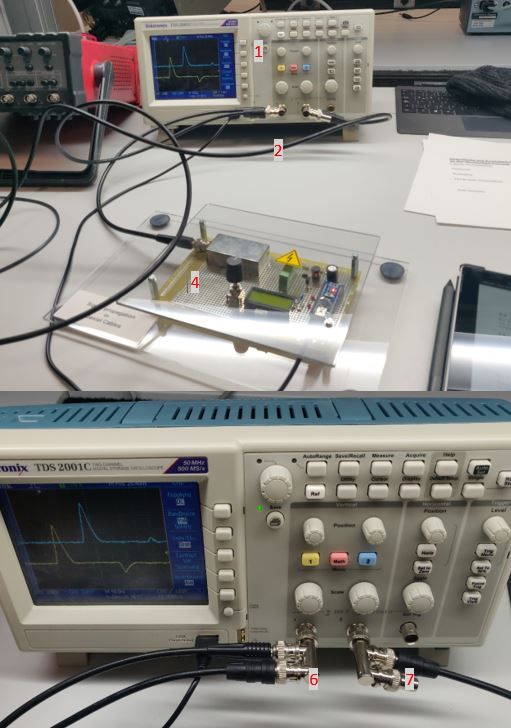
\includegraphics[width=.6\textwidth]{aufbau/setup_num.JPG}
        % \end{framed}
        %\includegraphics[width=12cm]{} % insert image (incl. numbering)
        \caption{Components needed for the experiment.}  
        \label{fig:setup}
    \end{figure}
    %
    \begin{enumerate}
        \item Oscilloscope
        \item Coaxial cables in three lengths
        % \item Coaxial cables with unknown length and internal fault
        \item Circuit board
        % \item Multimeter
        \item T-piece
        \item \SI{50}{\ohm} termination resistor
        % \item Termination box
        % \item Tape measure
    \end{enumerate}
    %
    A better overview of the circuit board will give the following \cref{fig:circuit_board}. Again, the components are listed
    below.
    %
    \begin{figure}[h]
        \centering
        % \begin{framed}
            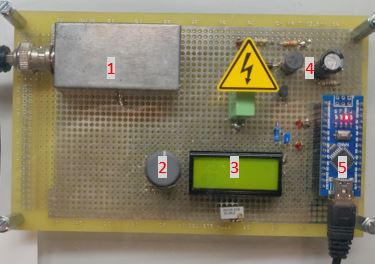
\includegraphics[width=.6\textwidth]{aufbau/circuit_board_num.JPG}
        % \end{framed}
        % \includegraphics[width=12cm]{} % insert image (incl. numbering)
        \caption{Detailed view on the circuit board.}  
        \label{fig:circuit_board}
    \end{figure}
    %
    \begin{enumerate}
        \item Pulse generator
        \item Potentiometer
        \item LCD
        \item Boost converter
        \item Arduino Nano Microcontroller board
    \end{enumerate}
    %
    The individual settings are explained in the execution chapter.